\documentclass[tikz]{standalone}
\usetikzlibrary{arrows}
\usepackage{amsmath}
\usepackage{amssymb}
\usepackage{mathrsfs}

\begin{document}

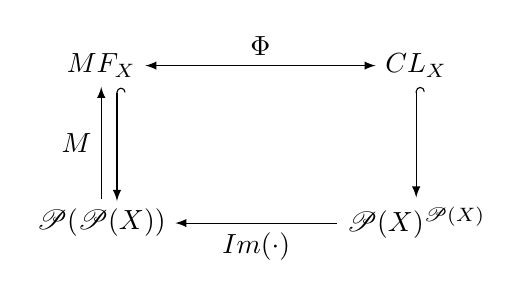
\begin{tikzpicture}[>=latex, scale=4]

% === NODES === (((
\node (a) at (0,0.5) {\(MF_X\)};
\node (b) at (0,0) {\(\mathscr{P} (\mathscr{P} (X))\)};
\node (c) at (1,0.5) {\(CL_X\)};
\node (d) at (1,0) {\(\mathscr{P} (X)^ {\mathscr{P} (X)}\)};
% )))

% === ARROWS === (((
\draw [->] (b) to node[left , midway] {\(M\)} (a);
\draw [<->] (a) to node[above , midway] {\(\Phi\)} (c);
\draw [right hook->] (c) -- (d);
\draw [->] (d) to node[below , midway] {\(Im(\cdot)\)} (b);
\draw [right hook->] (0.05,0.43) -- (0.05,0.07);
% )))

\end{tikzpicture}

\end{document}
